\documentclass{article}
\usepackage{graphicx}
\usepackage{caption}
\usepackage{subcaption}
\usepackage{natbib}
\usepackage{hyperref}
\usepackage{amsfonts}
\usepackage{amsmath}

\begin{document}

\title{Efficient Gibbs Sampling for Fields of Experts Image Models}

\author{Jonas Arnfred}

\maketitle

\section{Introduction}

\section{Method}

% This is about HOW I did stuff
% \subsection{Sampling from the posterior}

% Cite matthias somewhere

To analyse the performance of conjugate gradient on the FoE framework, I 
have implemented a denoise algorithm which uses FOE as an image prior.  
Instead of learning the model parameters myself, I have used the filters 
learned on natural images in \citep{uwe}. Given an image $\textbf{u} \in 
\mathbb{R}^n$, the FoE framework defines the probability density of an 
image \textbf{u} as:

\begin{equation}
	p(\textbf{u}; \Theta) = 
	\frac{1}{Z(\Theta)}e^{-\epsilon||\textbf{u}||^2/2} \prod_{r=1}^{R} 
	\prod_{i=1}^{n} t_r(s_{ri})
\end{equation}

where $s_{ri}$ is the circular convolution of $u$ with the filter $f_r$, 
$r = 1, \ldots , R$, $\,\Theta$ is a collection of model parameters 
($f_r, \alpha_r$, $\sigma_r$) and $Z$ is the partition function.  The 
potentials $t_r(s)$ used are mixtures of gaussians defined as:

\begin{equation}
	t_r(s) = \sum_{j=1}^{J} \alpha_{rj}\mathcal{N}(s|o, \sigma^2_{rj})
\end{equation}

where $J$ is the number of mixtures used in the model, $\alpha_{rj}$ is 
the scale for the $j$th gaussian and $\sigma^2_{rj}$ the variance. To 
sample from this density \citep{uwe} propose using an auxiliary-variable 
Gibbs sampler which introduces the indicator variables $z_{ri} \in {1, 
\ldots, J}^R$ that chooses the component of the mixture selected.  This 
way $t_r(s_{ri})$ given $z_{ri}$ is equivalent to a gaussian and much 
easier to sample from. Using Gibbs sampling we can alternate between 
sampling $\textbf{z}^{(t + 1)} \sim p(\textbf{z}|\textbf{u};\Theta)$ and 
$\textbf{u}^{(t + 1)} \sim p(\textbf{u}|\textbf{z};\Theta)$ where t is 
the current iteration.  With a little restructuring of (1) and (2) the 
conditionals for $\textbf{u}$
and $\textbf{z}$ are given by

\begin{equation}
	p(\textbf{z}_{ri}|\textbf{u};\Theta) \propto \alpha_{rz_{ri}} \times 
	\mathcal{N}(s|o, \sigma^2_{rz_{ri}})
\end{equation}

\begin{equation}
	p(\textbf{u}|\textbf{z};\Theta) \propto \mathcal{N}\left(\textbf{u}; 
	0, \left( \epsilon \textbf{I} + \sum_{i=1}^{R}B_r^T 
	diag(1/\sigma^2_{rz_{ri}}) B_r \right)^{-1} \right)
\end{equation}

where $B_r$ are the matrices that correspond to a convolution of 
$\textbf{u}$ with the filter $\textbf{f}_r$. To sample from 
$p(\textbf{u}|\textbf{z};\Theta)$ we sample $n_0 \sim \mathcal{N}(0, 
\textbf{I}) \in \mathbb{R}^{Rn}$. If we denote $\,A = \epsilon 
\textbf{I} + \sum_{i=1}^{R} B_r^T diag(1/\sigma^2_{rz_{ri}}) B_r\,$ and 
$\,n_1 = \sum_{i=1}^{R} B_r^T diag(1/\sigma^2_{rz_{ri}})\,$ we can then 
sample $u = A^{-1} n_1 \sim \mathcal{N}(0, A^{-1})$. Given the noisy 
image $\textbf{y}$ we can to sample the posterior for image denoising by

\begin{align}
	p(\textbf{u}| \textbf{y}, \textbf{z}; \Theta) & \propto 
	p(\textbf{y}|\textbf{u}) \cdot p(\textbf{u}|\textbf{z};\Theta) \\
	& \propto \mathcal{N} \left( \textbf{u} ; \, \tilde{A} y / \sigma^2, 
	\, \tilde{A}\right)
\end{align}

where $\tilde{A}$ is defined as $(\textbf{I}/\sigma^2 + A^{-1})^{-1}$.

This means that in order to sample from the posterior distribution we 
need to solve two linear systems: $\textbf{u} = \tilde{A}^{-1} \cdot 
n_1$ and $\textbf{u}_{\mu} = \tilde{A}^{-1} \cdot \textbf{y}/\sigma^2$.  
Since these two systems are solved for every iteration of the Gibbs 
sampling, it's important that they are solved fast for the algorithm to 
be efficient.  

\subsection{Optimizing for Conjugate Gradient}

The denoise algorithm proposed by \citep{uwe} uses choleski 
decomposition to solve the systems which doesn't scale well to images 
and doesn't provide much room for optimizations. The first step of 
speeding up the algorithm was thus to implement a Gibbs sampler that 
uses conjugate gradient. This allowed for several possible ways to 
increase the speed of the algorithm: Preconditioning, lower error 
tolerance, resizing of the scales ($\sigma^2_{rz_{ri}}$) and finally 
eliminating the more extreme values of the scales.

Since the goal of the implemented denoising algorithm is not to achieve 
superior denoising results, but rather serve as a tool for analysis, it 
differs from the implementation specified in \citep{uwe} on one account.  
Instead of running four Gibbs samplers concurrently, only one sampler is 
run.  This makes it more difficult to estimate when to stop the 
algorithm, so instead of using the variance in between the four 
concurrent samplers to estimate when to stop, I let the Gibbs sampler 
run for a set amount of conjugate gradient iterations. This facilitates 
analysis since the accumulated amount of conjugate gradient iterations 
provides a common atomic unit across different runs.

In order to speed up conjugate gradient we can use a preconditioner to 
improve the condition number of $A$. If are trying to solve the system 
$Ax = b$ and have a matrix $M$ for which $\kappa(M^{-1}A) \ll \kappa(A)$ 
then we can usually solve $Ax = b$ faster by solving $M^{-1}Ax = 
M^{-1}b$ instead \citep{pain}. The problem lies in finding an M which is 
invertible and in fact improves the condition number.

Alternatively (and much easier) we can increase how small the error must 
be before we stop iterating. This in turn means that we are accepting 
solutions that are futher from the true solution of the system which 
might negatively impact the quality of the denoising.

Instead of looking at the algorithm, it might prove useful to change 
parameters to create equations that are faster to solve. One way to do 
this is by changing the scales used in the gaussian mixture. In 
\citep{uwe} a fixed number of 15 scales is specified as $s = exp(0, 
\pm1, \ldots, \pm5, \pm7, \pm9)$. To scale $s$ I introduce a factor $p 
\in \{1, .95, .9, \ldots , 0.1\}$ in $s = exp(\ldots)^p$. This ensures 
that the more extreme scales are altered more than those in between.
%
%
%
% What do I want to write about?  First introduce the probabilistic 
% Model, then
% shortly go over how the gibbs sampling works

% Now go into depth with the systems I need to solve to denoise an image 

% Now introduce the differences from DARMSTADT and specify on what points my
% solution is different from theirs (Don't talk about why)

% Related to differences, talk about using cg instead of cholesky
% decomposition, about using number of conjugate gradient iterations to
% measure out the burn-in time. About how I'm only sampling from one image and
% not 4 per iteration. About how I'm stopping the process after a fixed number
% of iterations too.  Also talk about the burn-in samples are discarded and
% that the average of the samples that follow is the basis for the image

% Now talk about the experiments: How was the data collected?
% Talk about exclusions of scales
% Talk about variations or scalings of scales
% Talk about variations in CG cut-off rate (tolerance)
% Mention that the data is for one image only, and not averaged

% Show plot of 5 images with different sigma noise

\section{Results}

\begin{figure}[h]
		\begin{subfigure}[b]{0.19\textwidth}
                \centering
				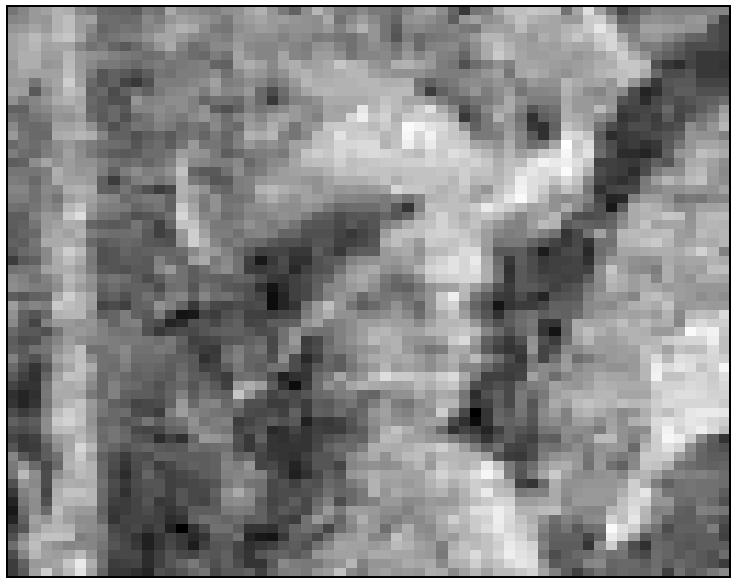
\includegraphics[width=\textwidth]{img/img_22_psnr}
				\caption{psnr of $\approx 22$}
				\label{psnr_22}
		\end{subfigure}%
		~ %add desired spacing between images, e. g. ~, \quad, \qquad 
		\begin{subfigure}[b]{0.19\textwidth}
                \centering
				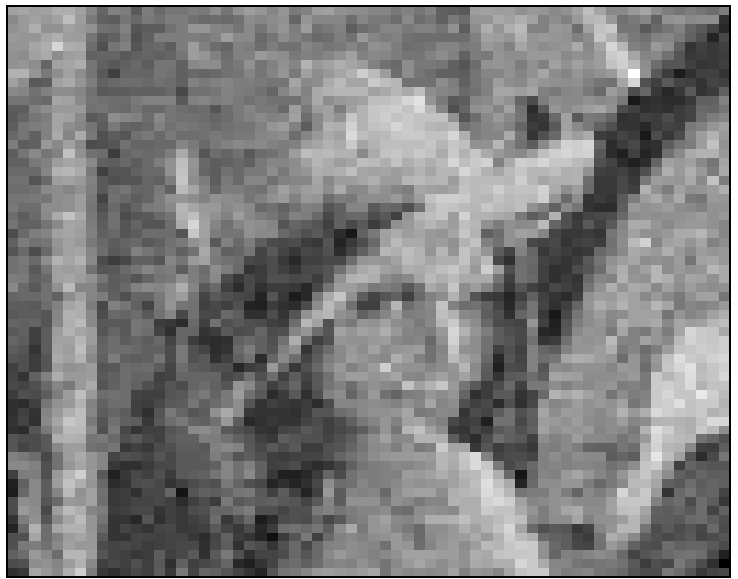
\includegraphics[width=\textwidth]{img/img_24_psnr}
				\caption{psnr of $\approx 24$}
				\label{psnr_24}
		\end{subfigure}%
		~ %add desired spacing between images, e. g. ~, \quad, \qquad 
		\begin{subfigure}[b]{0.19\textwidth}
                \centering
				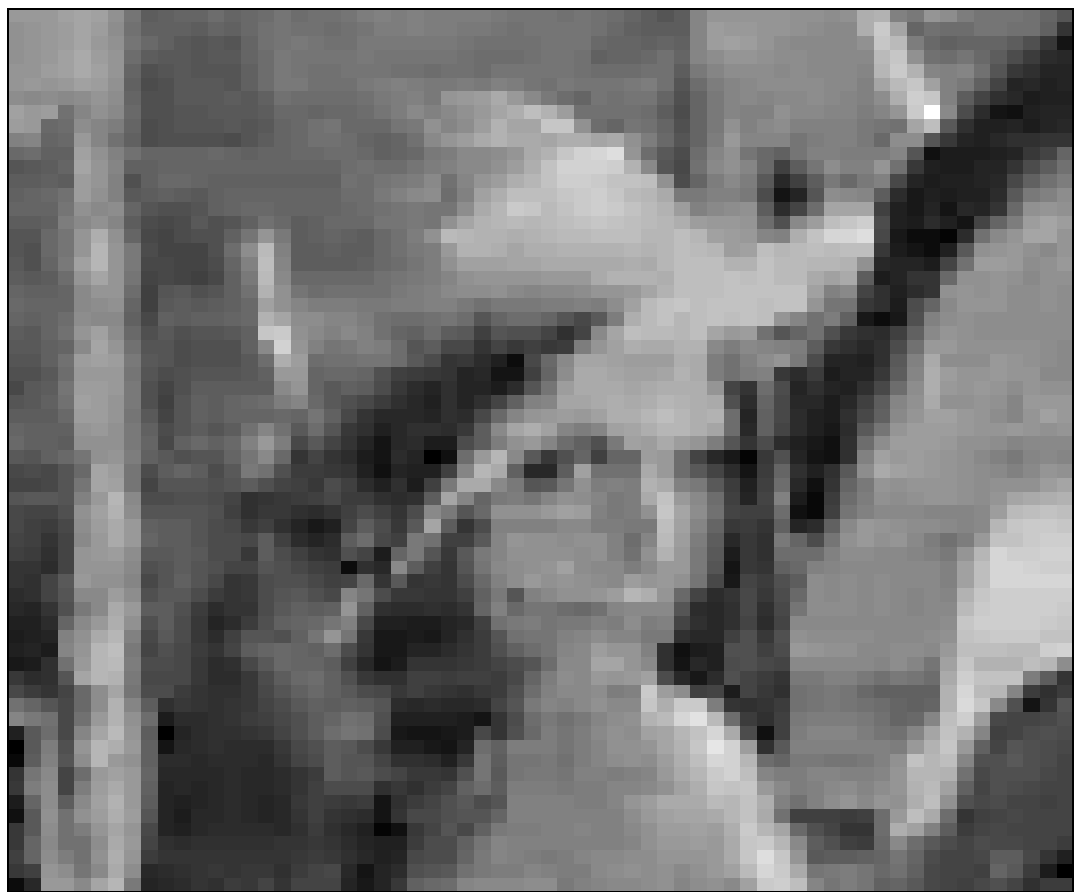
\includegraphics[width=\textwidth]{img/img_26_psnr}
				\caption{psnr of $\approx 26$}
				\label{psnr_26}
		\end{subfigure}%
		~ %add desired spacing between images, e. g. ~, \quad, \qquad 
		\begin{subfigure}[b]{0.19\textwidth}
                \centering
				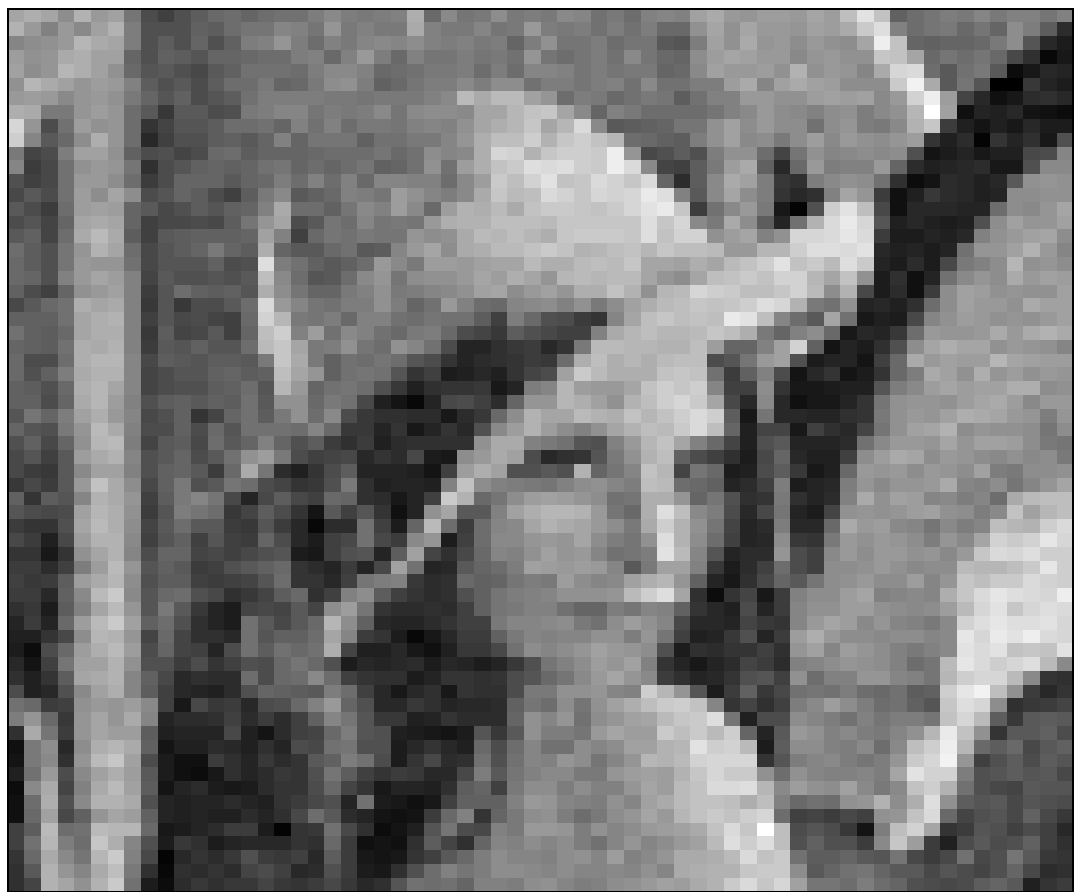
\includegraphics[width=\textwidth]{img/img_28_psnr}
				\caption{psnr of $\approx 28$}
				\label{psnr_28}
		\end{subfigure}%
		~ %add desired spacing between images, e. g. ~, \quad, \qquad 
		\begin{subfigure}[b]{0.19\textwidth}
                \centering
				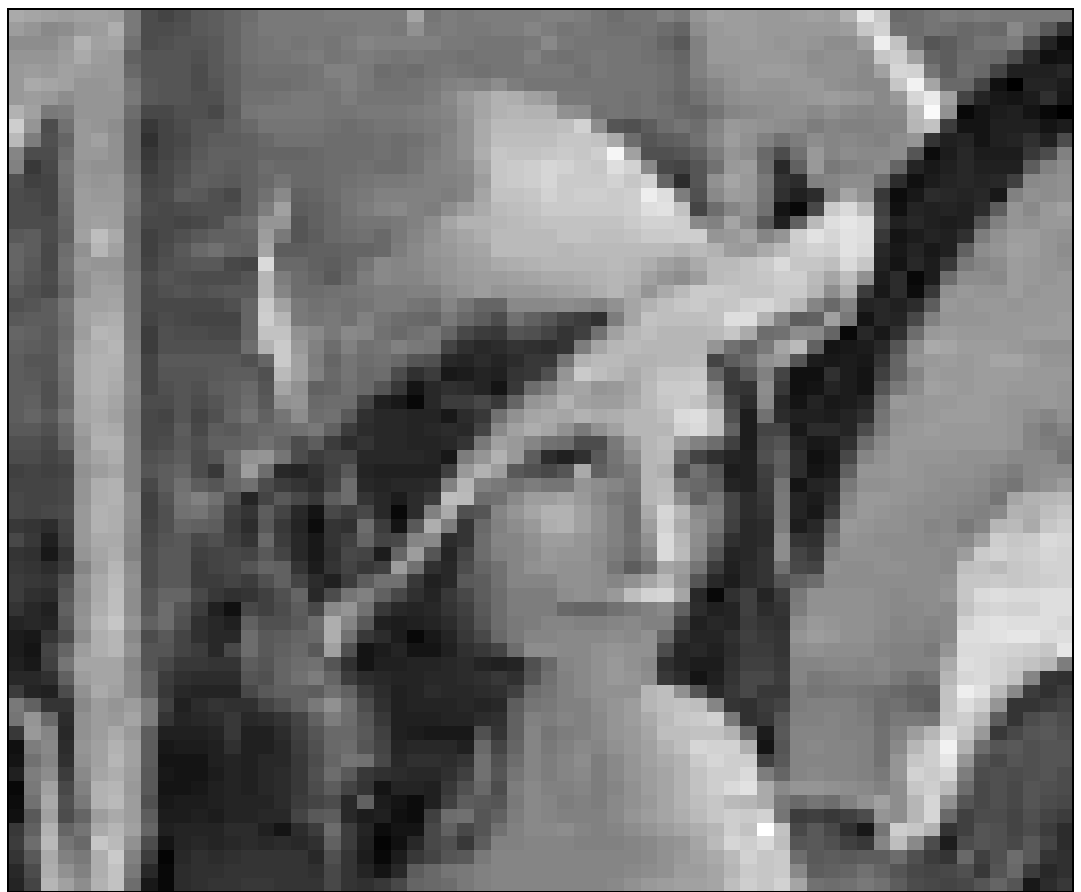
\includegraphics[width=\textwidth]{img/img_30_psnr}
				\caption{psnr of $\approx 30$}
				\label{psnr_30}
		\end{subfigure}%
		\caption{Examples of images at different psnr}
		\label{img_examples}
\end{figure}

To evaluate what different levels of signal to noise ratio (psnr) 
translates to in image quality, figure \ref{img_examples} showcases some 
examples for values typically encountered during the experiments. [Add 
psnr of noisy image at the three noise levels]. 


% This is about WHAT the stuff I did turned out to look like

% Introduce the plot of the sigma variations and make sure to explain the
% features of the plot. Explain the shading, the burn-in line, explain that
% even during burn-in, the psnr is of the average so far. Then analyse the
% data:
% 
% Figure 1
% - Note that this reflects a simple implementation of cg but with all original
%   (being from DARMSTADT) parameters unchanged.
% - Note how the the psnr as the average is lowered when it is reset to exclude
%   the first samples
% - Note very clearly that I'm showing iterations from the process of finding
%   the u_mu ONLY.

% Figure 2
% Now introduce the plot of the zoom, specifying the sigma it was taken at.
% - Note how the cg decays exponentially, and how there isn't much improvement
%   in psnr to be seen after the norm is smaller than 1.
% - Explain that this is a general example, and that it can been seen from figure1
% - Note how the psnr is at maximum early in the cg

% Figure 3 and 4
% Introduce the two figures with variation of tolerance to follow up on the last data
% - Mention the change in Y-axis.
% - Note how this data confirms that there isn't a big punishment for stopping cg early
% - Note also that there isn't much improvement either for higher noise levels

% Figure 5 Introduce the removal scales figure
% - Note how the original unremoved scales is higher than the rest during most
%   of the denoising process
% - Note how the data for removed scales shows that simulations hit a psnr
%   ceiling much faster when the scales are removed

% Figure 6 and 7 The scaled scales figure and heatmap
% - Introduce the data (how the figure 6 shows a smaller subset of figure 7)
% - Introduce the heatmap and explain that for each 100 iterations it shows the
%   maximum psnr value
% - Note how the pattern is similar to figure 5
% - Note how the spikes created close to the burn-in shows up around 1500 iterations

% Figure 

\section{Discussion}

% Talk about how the removal of scales and the rescaling of scales only applies
% to a limited situation, since the probabilistic model is trained with these
% specific scales in mind, so it's not impossible that a different model with
% fewer scales or smaller scales would fare better.

% Talk about how the fact that this data is based on a single image makes it
% volatile to changes. Talk about how the fixed burn-in rate might or might not
% be optimal.

% Discuss how the scaling is not doing anything constructive. We might get
% faster cg, which gives faster gibbs sampling steps, but in return it takes
% more steps for the gibbs sampling to reach the same psnr level, if possible
% at all

% Similarly with regards to removal of scales, it doesn't get us anywhere.

% In case we are willing to pay a bit in terms of optimal psnr it might however
% be interesting to change the tolerance of the cg. Here we can gain a steeper
% rate of psnr increase per iteration by being less strict about how precise we
% expect the end result of the cg, however this gain comes at a cost of lower
% optimal psnr, especially at higher noise rates

% It might make sense to look more deeply into the relationships between 
% conjugate gradient. I'll add a a plot

\section{Conclusion}

Write about how MRF isn't as useful if it's not fast, and how I've 
showed that to speed it up, we'll can't do anything without relearning 
the model when it comes to the scales. However we can change the 
conjugate gradient which for low noise can improve things quite a bunch.

% \input{introduction.tex}

% \input{method.tex}

% \input{results-discussion.tex}

% \input{conclusion.tex}

%\bibliographystyle{abbrv}
%\bibliography{bibliography}  

% \input{appendix.tex}

% \balancecolumns

% Bibliography
\bibliographystyle{unsrtnat}
\bibliography{yemen}

\end{document}
